\chapter{Background}
\section{Gravitational-wave}
\subsection{...}
\section{Sources of Gravitational-wave}
\subsection{...}
\section{Interferometric Gravitational-wave detection} \label{sec:13}

\subsection{Detection Principle}
地上の大型重力波検出器の基本要素はMichelson型レーザー干渉計である。プラスモードの重力波がFig.\ref{img:img}に示すようなMichelson型レーザー干渉計を垂直に通過する場合を考える。

\subsection{Michelson Interferometer}
\begin{figure}[H]
  \begin{center}   
    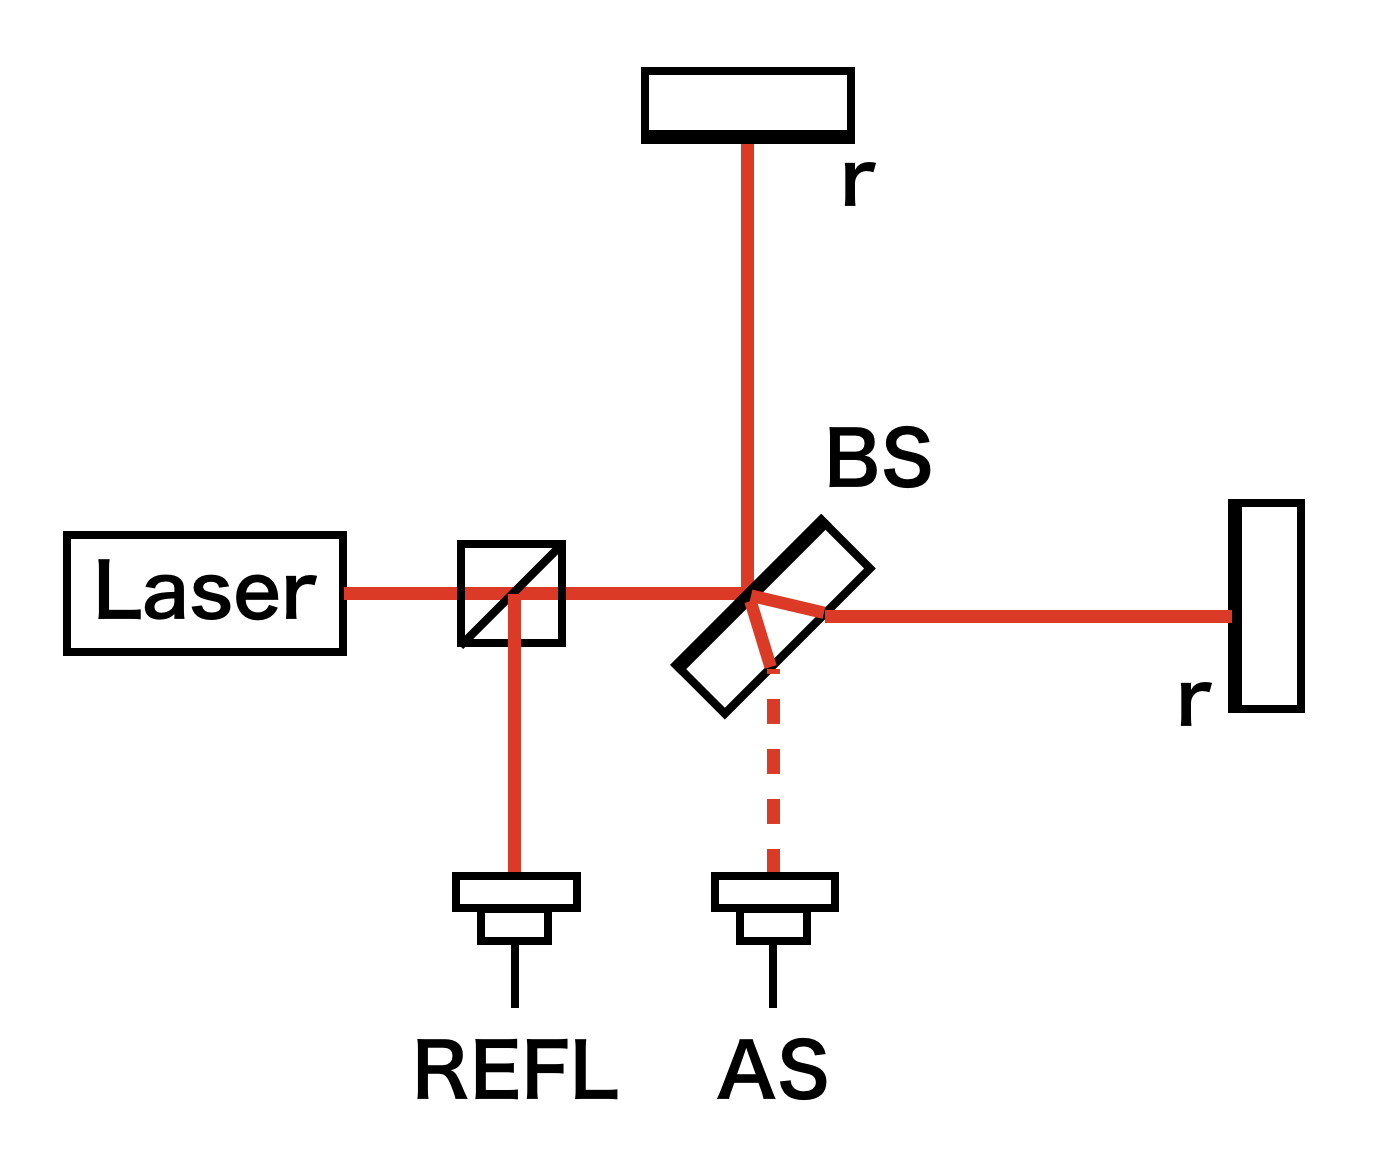
\includegraphics[width=8.0cm]{./img_chap1/img132.png}
    \caption{Michelson Interferometer. }\label{img:img132}
  \end{center}
\end{figure}

Michelson interferometer is a converter from the optical phase difference of two lights to the amplitude modulation of a single light. Consider about the interferometer shown in Fig. \ref{img:img132}. Incident light can be wrtten as,
\begin{eqnarray}
  E_{\mathrm{in}} = E_{0} e^{i\omega{t}},
\end{eqnarray}
where $E_0$ is the amplitude and $\omega_0$ is the angular frequency of the laser field
. Two lights splited by the Beam Spliter (BS) interferer at the Anti-symetric (AS) port and Refrection (REFL) port. The output fieled at the AS port is represented as,
\begin{eqnarray}
  E_{\mathrm{AS}} = -\frac{1}{2}rE_{0} e^{i\left(\omega_{0} t-\phi_{x}\right)}+\frac{1}{2}r E_{0} e^{i\left(\omega_{0} t-\phi_{y}\right)},
\end{eqnarray}
where $r$ denote the amplitude reflectivity of the end mirrors, and $\phi_{x}$ and $\phi_{x}$ are the phase delay due to the light traveling in the $x$ and $y$ arms. This output signal can be represented as a single fieled as,
\begin{eqnarray}
E_{\mathrm{AS}} = i r E_{0} e^{i\left(\omega_{0} t-\left(\phi_{x}+\phi_{y}\right) / 2\right)} \sin \left(\frac{\phi_{x}-\phi_{y}}{2}\right). \label{eq:eq132}
\end{eqnarray} 
Wwe find that the amplitude of the output light is a function of the difference between two phases; $\phi_{x}-\phi_{y}$. Furthermore, the power of output light at the AS port is obtained by squaring the Eq.\ref{eq:eq132}, 
\begin{eqnarray}
  P_{\mathrm{AS}} &=\left[r\sin({\phi_{-}})\right]^2P_0  \label{eq:eq133}
\end{eqnarray}
Similarly, power of the output light as REFL port is written as,
\begin{eqnarray}
  P_{\mathrm{REFL}} &=\left[(r\cos({\phi_{-}}))\right]^2P_0. \label{eq:eq134}
\end{eqnarray}
Therefore, we can measure the optical phase difference as the amplitude changes using a Photo Detector (PD) and detect GWs.

\subsection{Sensing Noise}
テストマスが自由質点として外乱を受けていない理想的な場合には、Michelson干渉計のレーザー光の強度ゆらぎと周波数ゆらぎ、検出器でのショットノイズが感度を制限する。

\subsubsection{Noise Contribution}
\begin{eqnarray}
  \Delta{\phi_{-}} = \frac{\tan{(\phi_{-})}}{2} \left[\left(\frac{\Delta P_{\mathrm{AS}}}{P_{\mathrm{AS}}}\right) + \left(\frac{\Delta{P_0}}{P_0}\right) \right] 
\end{eqnarray}

$\phi_{-}=\frac{4\pi{L_{-}}}{\lambda}$なので
\begin{eqnarray}
  h = \frac{\Delta{L_{-}}}{L} = \frac{\lambda}{4\pi{L}}\Delta{\phi_{-}} + \frac{L_{-}}{L}\left(\frac{\Delta{f}}{f}\right)
\end{eqnarray}

\begin{eqnarray}
  h = \frac{\lambda}{8\pi{L}}\tan{(\phi_{-})} \left[\left(\frac{\Delta P_{\mathrm{AS}}}{P_{\mathrm{AS}}}\right) + \left(\frac{\Delta{P_0}}{P_0}\right) \right] + \frac{L_{-}}{L}\left(\frac{\Delta{f}}{f}\right) \label{eq:eq137}
\end{eqnarray} 
となる。Eq.(\ref{eq:eq137})は、検出可能なひずみの大きさを小さくするには、以下のことが必要である。
\begin{itemize}
  \setlength{\itemsep}{1pt}      %2. ブロック間の余白
  \setlength{\parskip}{-1pt}     %4. 段落間余白.
  \setlength{\itemindent}{0pt}   %5. 最初のインデント
  \setlength{\labelsep}{5pt}     %6. item と文字の間  
\item 光検出の誤差$(\Delta P_{\mathrm{AS}}/P_{\mathrm{AS}})$とレーザーの光量ゆらぎ$\Delta{P_0}/P_0$からの寄与を小さくするには、$\phi_{-}\to0$にすべきである。これはASポートをダークにすることを意味する。
\item 周波数ゆらぎ$\Delta{f}/f$からの寄与を小さくするには、腕の非対称さ$L_{0}\to0$にすべきである。
\end{itemize}

\subsubsection{Detection Noise}
Eq.(\ref{eq:eq137})によれば、検出誤差の寄与を小さくするには$\tan{(\phi_{-})}\to0$になるようにASポートでの干渉縞を暗縞にすればよく、


光検出器で光のパワーを検出する場合、ショットノイズと呼ばれる、光子数のゆらぎに起因するノイズをもつ。光子数のカウントはポアソン分布にしたがうが、光子数$N$が十分に大きい場合標準偏差$\sqrt{N}$のガウス分布に従う。つまり光検出器にパワー$P$の光が入射した場合、このショットノイズは
\begin{eqnarray}
  P_{\mathrm{shot}} \propto \sqrt{P}\ \ [W/\sqrt{\mathrm{Hz}}]  \label{eq:eq136}
\end{eqnarray}
のようなホワイトノイズをもち、ASポートでのパワーの平方根に比例したノイズをもつ。


相対誤差はパワーの平方根に逆比例する。さらにEq.(\ref{eq:eq133})より、光検出の相対誤差は
\begin{eqnarray}
  \frac{\Delta P_{\mathrm{AS}}}{P_{\mathrm{0}}}  \propto \frac{1}{\sqrt{P_{\mathrm{AS}}}}\ \ [1/\sqrt{\mathrm{Hz}}]  \label{eq:eq136}
\end{eqnarray}
にように、Michelson干渉計へ入射した光量の平方根に反比例することがわかる。つまりショットノイズ


検出ノイズがひずみ検出に与える影響は、Eq.(\ref{eq:eq137})より、ASポートにおいた光検出器に入射するパワーの相対ゆらぎ$(\Delta P_{\mathrm{AS}}/P_{\mathrm{AS}})$で与えられる。この相対ゆらぎは、パワーの平方根に反比例するので、ASポートに入射する

\subsection{Disturbance on the Test Mass}
テストマスはさまざまな外乱によって振動しており、この振動は重力波検出においてのノイズとなる。

\subsubsection{Seismic Noise}
地面振動は地上の重力波検出器においてもっとも振幅が大きい外乱である。さまざまな励起源からの弾性波が地面や構造物をつたわってテストマスを揺らす。そのため地面振動を低減するには、励起源から離れた静かな場所でテストマスを防振することが必要である。

\subsubsection{Newtonian Noise}
Newtonian Noise は、重力勾配ノイズとも呼ばれ、周囲の物体の密度ゆらぎが重力相互作用でテストマスを揺らすノイズである。この密度ゆらぎは地面を伝わる弾性波によって生じ、それが遠隔作用で空間を伝わるため防振することはできない。現在の第二世代の重力波検出器の感度では問題にはならないが、第3世代では10Hz周辺の感度を制限するとされている。

Newtonianノイズを低減するには、地震計アレイをもちいたFeedforward制御が提案されている。

\subsubsection{Thermal Noise}
外部からの外乱以外にも、鏡の基材や表面の粒子がランダムな熱運動をして変位雑音を生み出す。この熱雑音は、1) mirror thermal noise 2) mirror coating thermal noise 3) suspension thermal noise の3つにわけることができる\cite{dan2016study}。

温度$T$をもつ鏡の Mirror thermal noise の変位雑音は、
\begin{eqnarray}
  G_{\mathrm{SB}}(f)=\frac{4 k_{B} T}{\omega} \frac{1-\sigma^{2}}{\sqrt{\pi} E w_{0}} \phi_{\mathrm{sub}}(f)
  \label{eq:eq140}
\end{eqnarray}
のように与えられる\cite{levin1998internal,numata2003wide}。ここで$k_{B}$はボルツマン定数、$\omega$は角周波数、$\sigma$,$E$は基材のポアソン比、ヤング率であり、$\phi_{\mathrm{sub}}$ は鏡の基材のmechanical loss angle、$\omega_0$はビーム半径である。Eq.(\ref{eq:eq140})からわかるように、この熱雑音を低減するには温度を下げるかビーム径を大きくすればよい。

鏡の熱雑音は基材よりもむしろ表面のコーティングで制限される。Corting thermal noise の変位雑音は、
\begin{eqnarray}
G_{\mathrm{CB}}(f)=G_{\mathrm{SB}}(f)\left(1+\frac{2}{\sqrt{\pi}} \frac{1-2 \sigma}{1-\sigma} \frac{\phi_{\mathrm{coat}}}{\phi_{\mathrm{sub}}} \frac{d}{w_{0}}\right)
\end{eqnarray}
で与えられる\cite{numata2003wide,harry2002thermal}。ここで、$d$,$\phi_{\mathrm{coat}}$はそれぞれコーティングの厚さ、loss angle である。

そして最後に、鏡自身の




\subsubsection{Resudual Gas Noise}


\section{Large-scale Terrestrial Laser Interferometers}
\subsection{Overview}
地上検出器の最終的な目標は、第3世代と呼ばれる、基線長が数10kmの

地上検出器の最終的な目標は、第3世代とよばれる、数10kmの長期線検出器である。

そのために必要な要素技術の開発と実証のためにさまざまな検出器がつくられてきた。それらをTable\ref{tb:tb101}に示す\cite{chen2017brief}。

第1世代検出器(TAMA\cite{ando2001stable}, GEO\cite{grote2010geo}, LIGO\cite{abbott2009ligo}, Virgo\cite{accadia2012virgo})は、

第2世代検出器(KAGRA\cite{akutsu2018kagra}, Advanced Virgo\cite{acernese2014advanced}, Advanced LIGO\cite{aasi2015advanced})


\begin{table}[h] 
  \begin{center}
    \caption{\cite{chen2017brief,beker2013low}}\label{tb:tb101}
    \begin{tabular}{llll} 
      \hline
      Project & Baseline [km] & Effective Length [km] & Bedrock \\ \hline \hline
      LISM  & 0.02    & 32  & Granite/gneiss \\
      CLIO  & 0.1   & 190 & Granite/gneiss \\
      TAMA  & 0.3   & 96  & - \\ 
      GEO   & 0.6   & 1.2 & Sedimentary rock \\
      KAGRA   & 3  & 2850  & Granite/gneiss \\
      LIGO L1 & 4  & 1150  & Sedimentary soil \\
      LIGO H1 & 4  & 1150  & Sedimentary rock \\
      Virgo   & 3  & 850   & Sedimentary rock \\
      ET      & 10 & 3200  & - \\
      \hline
    \end{tabular}
  \end{center}
\end{table}

\subsection{Proto Type Interferometers of KAGRA}
\subsubsection{LISM}
LISMは世界で初めて地下に建設された20mのレーザー干渉計型の重力波検出器をつかって、干渉計の安定した運転を地下環境で実証するプロジェクトである。LISMの干渉計は20mのFabry-Perot光共振器を腕にもつマイケルソン型レーザー干渉計である。この腕共振器のフィネスは25000と非常に大きくCavity Pole は150Hzに相当する。このようにフィネスの大きい共振器にもかかわらず、DutyCycleは$99.8\,\%$であった。

安定稼働の大きな要因としては地面振動の同相雑音除去効果が考えられる。Fig.\ref{img:img122}にLISMの感度曲線を示す。懸架システムの伝達関数をもちいて計算された干渉計への地面振動の寄与と比較すると、地面振動の垂直方向成分が100Hz以下の感度を制限していることがわかるが、特筆すべきは6Hz以下の干渉計の感度が地面振動の寄与よりも小さいことである。これは、神岡の地下岩盤が十分に固く、低周波では20mの基線を一枚岩のようにうごかし基線長が低減される。このおかげで腕共振器が安定してロックでき、安定した干渉計の稼働が実現できた。
\begin{figure}[h]
  \begin{center}   
    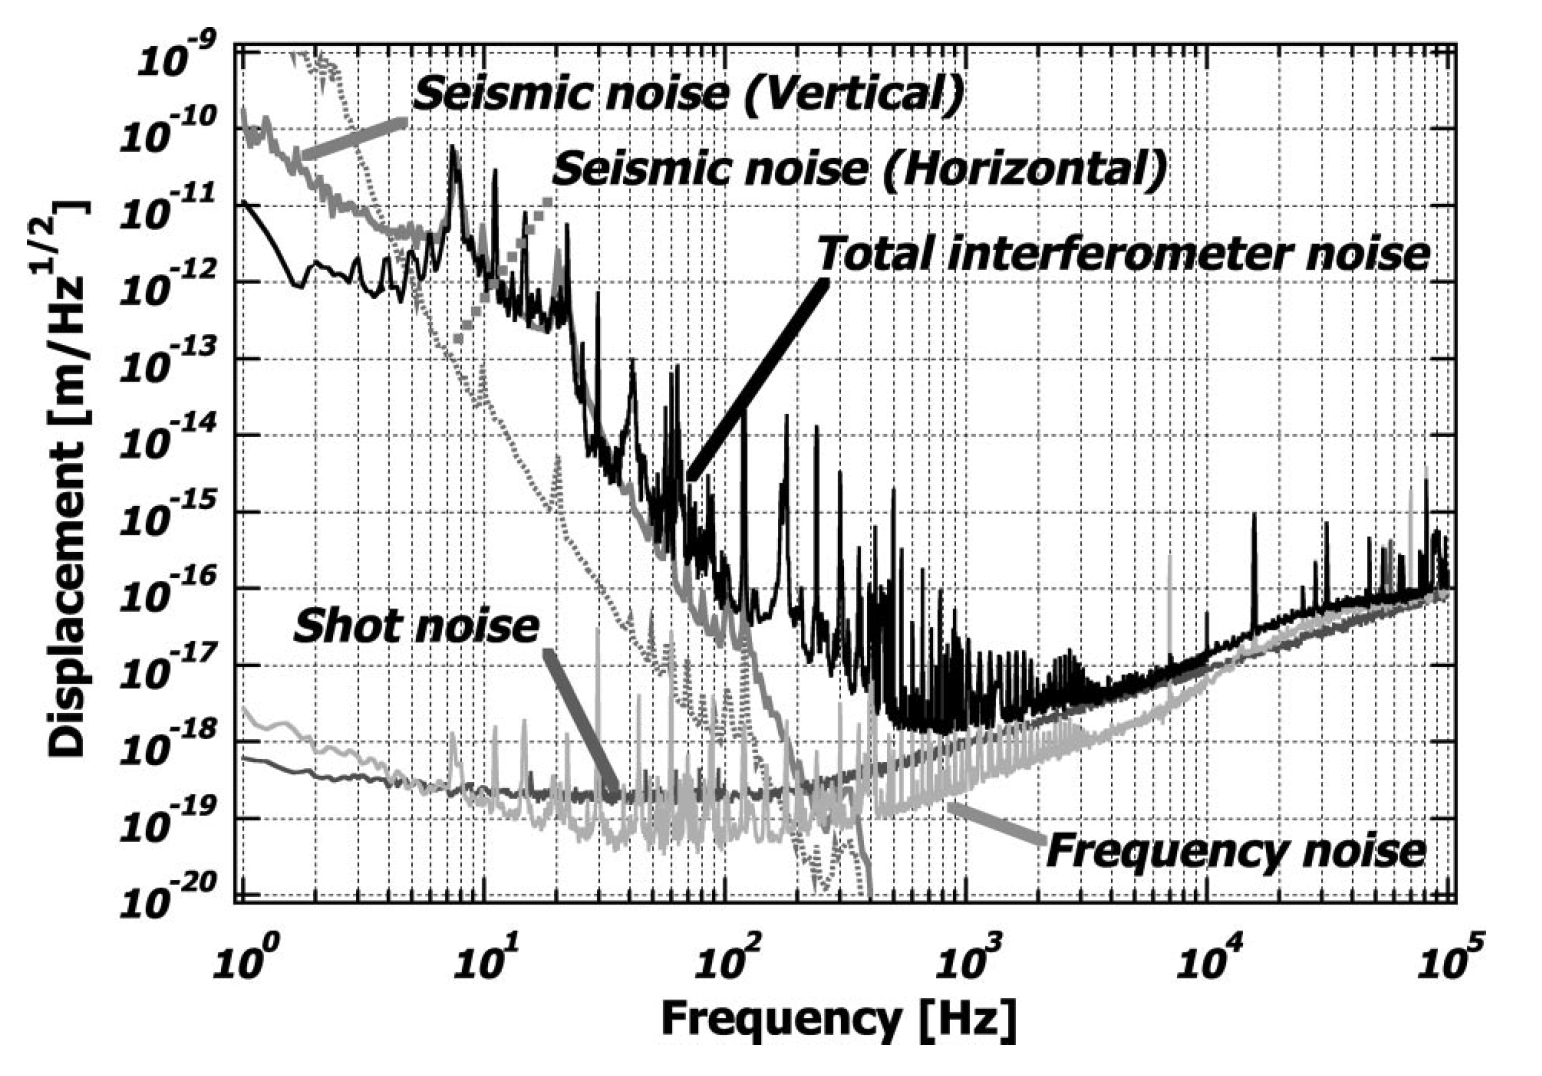
\includegraphics[width=12cm,height=7cm]{./img_chap1/img122.png}
    \caption{The noise equivalent detector sensitivity of LISM. This figure is cited from figure 5 in \cite{sato2004ultrastable}. } \label{img:img122}
  \end{center}
\end{figure}

\subsubsection{CLIO}
CLIOは、LISMに引き続いて地下に建設された100mのレーザー干渉計型重力波検出器であり、この検出器の目的は極低温に冷やした鏡を用いて熱雑音の低減を実証することである\cite{ohashi2003design}。そのために、地面振動が静かな地下環境で、熱伝導特性の良いサファイアでFabry−Pert光共振器を構築し、低振動なパルス管冷凍機\cite{tomaru2004development}を使用して20Kまで冷却をしている。このおかげで、室温での熱雑音で制限されていた干渉計の感度を低音鏡にして低減することができた\cite{uchiyama2012reduction}。

\begin{figure}[h]
  \begin{center}   
    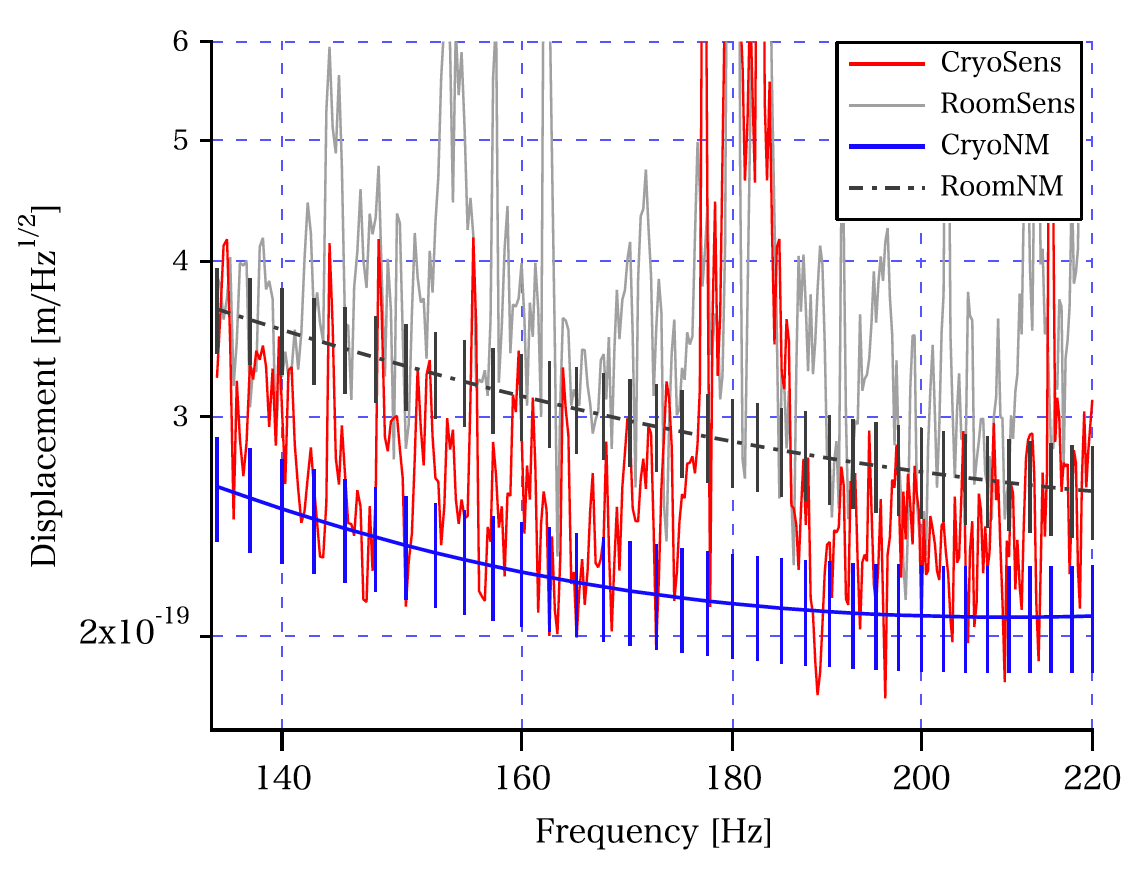
\includegraphics[width=12cm,height=7cm]{./img_chap1/img123.png}
    \caption{This figure is cited from figure 2 in \cite{uchiyama2012reduction}. } \label{img:img123}
  \end{center}
\end{figure}

\subsection{KAGRA}
\section{Theis Outline}

\section{Summary of the Chapter}
